\documentclass[12pt,letterpaper]{article}
\usepackage{graphicx,textcomp}
\usepackage{natbib}
\usepackage{setspace}
\usepackage{fullpage}
\usepackage{color}
\usepackage[reqno]{amsmath}
\usepackage{amsthm}
\usepackage{fancyvrb}
\usepackage{amssymb,enumerate}
\usepackage[all]{xy}
\usepackage{endnotes}
\usepackage{lscape}
\newtheorem{com}{Comment}
\usepackage{float}
\usepackage{hyperref}
\newtheorem{lem} {Lemma}
\newtheorem{prop}{Proposition}
\newtheorem{thm}{Theorem}
\newtheorem{defn}{Definition}
\newtheorem{cor}{Corollary}
\newtheorem{obs}{Observation}
\usepackage[compact]{titlesec}
\usepackage{dcolumn}
\usepackage{tikz}
\usetikzlibrary{arrows}
\usepackage{multirow}
\usepackage{xcolor}
\newcolumntype{.}{D{.}{.}{-1}}
\newcolumntype{d}[1]{D{.}{.}{#1}}
\definecolor{light-gray}{gray}{0.65}
\usepackage{url}
\usepackage{listings}
\usepackage{color}

\definecolor{codegreen}{rgb}{0,0.6,0}
\definecolor{codegray}{rgb}{0.5,0.5,0.5}
\definecolor{codepurple}{rgb}{0.58,0,0.82}
\definecolor{backcolour}{rgb}{0.95,0.95,0.92}

\lstdefinestyle{mystyle}{
	backgroundcolor=\color{backcolour},   
	commentstyle=\color{codegreen},
	keywordstyle=\color{magenta},
	numberstyle=\tiny\color{codegray},
	stringstyle=\color{codepurple},
	basicstyle=\footnotesize,
	breakatwhitespace=false,         
	breaklines=true,                 
	captionpos=b,                    
	keepspaces=true,                 
	numbers=left,                    
	numbersep=5pt,                  
	showspaces=false,                
	showstringspaces=false,
	showtabs=false,                  
	tabsize=2
}
\lstset{style=mystyle}
\newcommand{\Sref}[1]{Section~\ref{#1}}
\newtheorem{hyp}{Hypothesis}

\title{Problem Set 3}
\date{Due: November 20, 2022}
\author{Applied Stats/Quant Methods 1}


\begin{document}
	\maketitle
	\section*{Instructions}
	\begin{itemize}
		\item Please show your work! You may lose points by simply writing in the answer. If the problem requires you to execute commands in \texttt{R}, please include the code you used to get your answers. Please also include the \texttt{.R} file that contains your code. If you are not sure if work needs to be shown for a particular problem, please ask.
	\item Your homework should be submitted electronically on GitHub.
	\item This problem set is due before 23:59 on Sunday November 20, 2022. No late assignments will be accepted.
	\item Total available points for this homework is 80.
	\end{itemize}

		\vspace{.25cm}
	
\noindent In this problem set, you will run several regressions and create an add variable plot (see the lecture slides) in \texttt{R} using the \texttt{incumbents\_subset.csv} dataset. Include all of your code.

	\vspace{.5cm}
\section*{Question 1}
\vspace{.25cm}
\noindent We are interested in knowing how the difference in campaign spending between incumbent and challenger affects the incumbent's vote share. 
	\begin{enumerate}
		\item Run a regression where the outcome variable is \texttt{voteshare} and the explanatory variable is \texttt{difflog}.	\vspace{1cm} \\
		\noindent The following code was used to run the regression: \\
		\lstinputlisting[language=R, firstline=39, lastline=39]{code/PS3.R}
		\noindent From this, using Stargazer an output table was created (see Table 1)
		\begin{table}[!htbp] \centering 
			\caption{Difflog and Voteshare} 
			\label{} 
			\begin{tabular}{@{\extracolsep{5pt}}lc} 
				\\[-1.8ex]\hline 
				\hline \\[-1.8ex] 
				& \multicolumn{1}{c}{\textit{Dependent variable:}} \\ 
				\cline{2-2} 
				\\[-1.8ex] & voteshare \\ 
				\hline \\[-1.8ex] 
				difflog & 0.042$^{***}$ \\ 
				& (0.001) \\ 
				& \\ 
				Constant & 0.579$^{***}$ \\ 
				& (0.002) \\ 
				& \\ 
				\hline \\[-1.8ex] 
				Observations & 3,193 \\ 
				R$^{2}$ & 0.367 \\ 
				Adjusted R$^{2}$ & 0.367 \\ 
				Residual Std. Error & 0.079 (df = 3191) \\ 
				F Statistic & 1,852.791$^{***}$ (df = 1; 3191) \\ 
				\hline 
				\hline \\[-1.8ex] 
				\textit{Note:}  & \multicolumn{1}{r}{$^{*}$p$<$0.1; $^{**}$p$<$0.05; $^{***}$p$<$0.01} \\ 
			\end{tabular} 
		\end{table}
		\noindent From this regression, there was a significant result between the 'difflog' and 'voteshare' variables, \textit{F}(1, 3191) = 1,852.791, \textit{p} $<$ .01, with R$^{2}$ = 0.367. This means that 36.7\% of the variance in the 'Voteshare' variable can be explained by the variance in the 'difflog' variable.
		\item Make a scatterplot of the two variables and add the regression line. 	\vspace{1cm} \\
		\noindent A scatterplot was made using the following code:
		\lstinputlisting[language=R, firstline=43, lastline=47]{code/PS3.R}
		\begin{figure}[h!]\centering
			\caption{\footnotesize Scatterplot of 'voteshare' and 'difflog'}
			\label{fig:plots}
			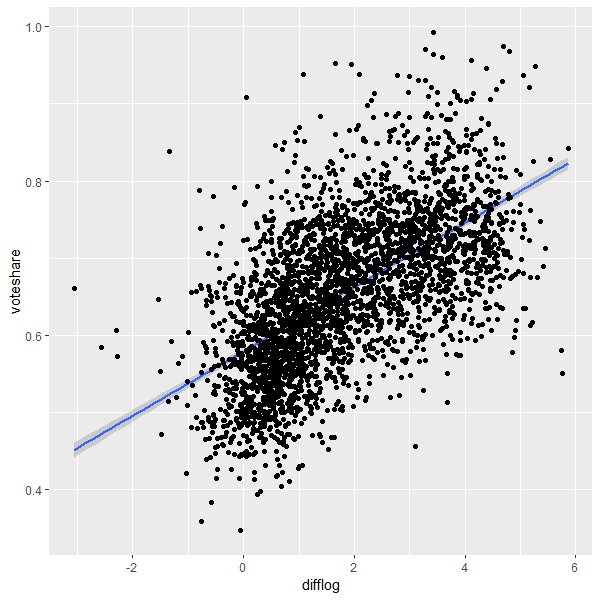
\includegraphics[width=.75\textwidth]{output/Reg1.png}
		\end{figure}
		\item Save the residuals of the model in a separate object.	\vspace{1cm} \\
		\noindent Residuals were saved using the following line:
		\lstinputlisting[language=R, firstline=50, lastline=50]{code/PS3.R}
		\item Write the prediction equation. \\
		\noindent According to the output table, for every increase in one unit in the 'difflog' variable, there is a 0.042 unit increase in 'voteshare'. This is shown via the equation: \\
		\noindent \textit{Y}$_{i}$ = 0.579 + 0.042\textit{X}$_{i}$
	\end{enumerate}
	
\newpage

\section*{Question 2}
\noindent We are interested in knowing how the difference between incumbent and challenger's spending and the vote share of the presidential candidate of the incumbent's party are related.	\vspace{.25cm}
	\begin{enumerate}
		\item Run a regression where the outcome variable is \texttt{presvote} and the explanatory variable is \texttt{difflog}.	\vspace{1cm} \\
		\noindent The following code was used to run the regression: \\
		\lstinputlisting[language=R, firstline=56, lastline=56]{code/PS3.R}
		\noindent From this, using Stargazer an output table was created (see Table 2)
		\begin{table}[!htbp] \centering 
			\caption{Difflog and Presvote} 
			\label{} 
			\begin{tabular}{@{\extracolsep{5pt}}lc} 
				\\[-1.8ex]\hline 
				\hline \\[-1.8ex] 
				& \multicolumn{1}{c}{\textit{Dependent variable:}} \\ 
				\cline{2-2} 
				\\[-1.8ex] & presvote \\ 
				\hline \\[-1.8ex] 
				difflog & 0.024$^{***}$ \\ 
				& (0.001) \\ 
				& \\ 
				Constant & 0.508$^{***}$ \\ 
				& (0.003) \\ 
				& \\ 
				\hline \\[-1.8ex] 
				Observations & 3,193 \\ 
				R$^{2}$ & 0.088 \\ 
				Adjusted R$^{2}$ & 0.088 \\ 
				Residual Std. Error & 0.110 (df = 3191) \\ 
				F Statistic & 307.715$^{***}$ (df = 1; 3191) \\ 
				\hline 
				\hline \\[-1.8ex] 
				\textit{Note:}  & \multicolumn{1}{r}{$^{*}$p$<$0.1; $^{**}$p$<$0.05; $^{***}$p$<$0.01} \\ 
			\end{tabular} 
		\end{table} 
		\noindent From this regression, there was a significant result between the 'difflog' and 'presvote' variables, \textit{F}(1, 3191) = 307.715, \textit{p} $<$ .01, with R$^{2}$ = 0088. This means that 8.8\% of the variance in the 'Presvote' variable can be explained by the variance in the 'difflog' variable.
		\item Make a scatterplot of the two variables and add the regression line. 	\vspace{1cm} \\
		\noindent A scatterplot was made using the following code:
		\lstinputlisting[language=R, firstline=60, lastline=64]{code/PS3.R}
		\begin{figure}[h!]\centering
			\caption{\footnotesize Scatterplot of 'presvote' and 'difflog'}
			\label{fig:plots}
			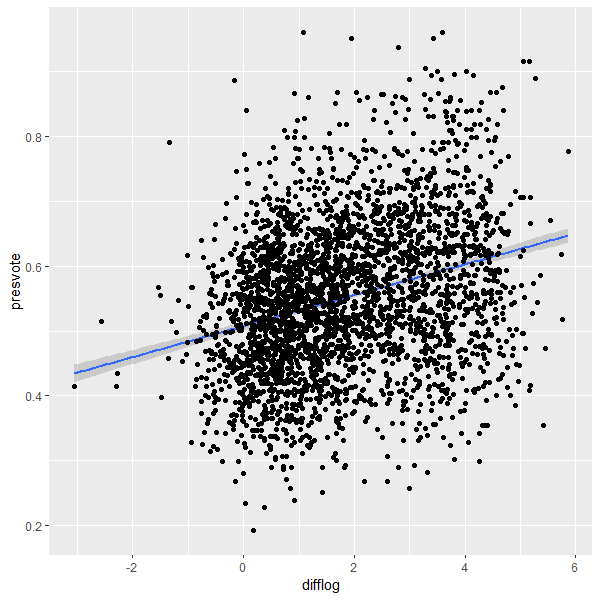
\includegraphics[width=.75\textwidth]{output/Reg2.png}
		\end{figure}
	\vspace{12cm} 
		\item Save the residuals of the model in a separate object.	\vspace{1cm} \\
		\noindent Residuals were saved using the following line:
		\lstinputlisting[language=R, firstline=67, lastline=67]{code/PS3.R}
		\item Write the prediction equation. \\
		\noindent According to the output table, for every increase in one unit in the 'difflog' variable, there is a 0.024 unit increase in 'voteshare'. This is shown via the equation: \\
		\noindent \textit{Y}$_{i}$ = 0.508 + 0.024\textit{X}$_{i}$
	\end{enumerate}
	
	\newpage	
\section*{Question 3}

\noindent We are interested in knowing how the vote share of the presidential candidate of the incumbent's party is associated with the incumbent's electoral success.
	\vspace{.25cm}
	\begin{enumerate}
		\item Run a regression where the outcome variable is \texttt{voteshare} and the explanatory variable is \texttt{presvote}.
			\vspace{1cm} \\
			\noindent The following code was used to run the regression: \\
		\lstinputlisting[language=R, firstline=73, lastline=73]{code/PS3.R}
		\noindent From this, using Stargazer an output table was created (see Table 3)
	\begin{table}[!htbp] \centering 
		\caption{Presvote and Voteshare} 
		\label{} 
		\begin{tabular}{@{\extracolsep{5pt}}lc} 
			\\[-1.8ex]\hline 
			\hline \\[-1.8ex] 
			& \multicolumn{1}{c}{\textit{Dependent variable:}} \\ 
			\cline{2-2} 
			\\[-1.8ex] & voteshare \\ 
			\hline \\[-1.8ex] 
			presvote & 0.388$^{***}$ \\ 
			& (0.013) \\ 
			& \\ 
			Constant & 0.441$^{***}$ \\ 
			& (0.008) \\ 
			& \\ 
			\hline \\[-1.8ex] 
			Observations & 3,193 \\ 
			R$^{2}$ & 0.206 \\ 
			Adjusted R$^{2}$ & 0.206 \\ 
			Residual Std. Error & 0.088 (df = 3191) \\ 
			F Statistic & 826.950$^{***}$ (df = 1; 3191) \\ 
			\hline 
			\hline \\[-1.8ex] 
			\textit{Note:}  & \multicolumn{1}{r}{$^{*}$p$<$0.1; $^{**}$p$<$0.05; $^{***}$p$<$0.01} \\ 
		\end{tabular} 
	\end{table}
		\noindent From this regression, there was a significant result between the 'voteshare' and 'presvote' variables, \textit{F}(1, 3191) = 826.950, \textit{p} $<$ .01, with R$^{2}$ = 0.206 This means that 20.6\% of the variance in the 'Voteshare' variable can be explained by the variance in the 'Presvote' variable.
		\item Make a scatterplot of the two variables and add the regression line. 
			\vspace{1cm} \\
			\noindent A scatterplot was made using the following code:
		\lstinputlisting[language=R, firstline=77, lastline=81]{code/PS3.R}
		\begin{figure}[h!]\centering
			\caption{\footnotesize Scatterplot of 'voteshare' and 'presvote'}
			\label{fig:plots}
			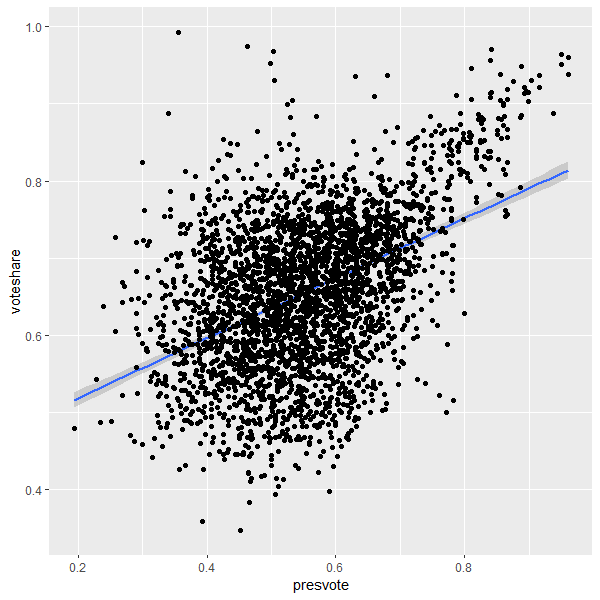
\includegraphics[width=.75\textwidth]{output/Reg3.png}
		\end{figure}
	\vspace{12cm} 
		\item Write the prediction equation. \\
			\noindent According to the output table, for every increase in one unit in the 'presvote' variable, there is a 0.388 unit increase in 'voteshare'. This is shown via the equation: \\
		\noindent \textit{Y}$_{i}$ = 0.441 + 0.388\textit{X}$_{i}$
	\end{enumerate}
	

\newpage	
\section*{Question 4}
\noindent The residuals from part (a) tell us how much of the variation in \texttt{voteshare} is $not$ explained by the difference in spending between incumbent and challenger. The residuals in part (b) tell us how much of the variation in \texttt{presvote} is $not$ explained by the difference in spending between incumbent and challenger in the district.
	\begin{enumerate}
		\item Run a regression where the outcome variable is the residuals from Question 1 and the explanatory variable is the residuals from Question 2.	\vspace{1cm} \\
		\noindent The following code was used to run the regression: \\
		\lstinputlisting[language=R, firstline=88, lastline=88]{code/PS3.R}
		\noindent From this, using Stargazer an output table was created (see Table 4)
		\begin{table}[!htbp] \centering 
			\caption{Residuals of Reg1 and Reg2} 
			\label{} 
			\begin{tabular}{@{\extracolsep{5pt}}lc} 
				\\[-1.8ex]\hline 
				\hline \\[-1.8ex] 
				& \multicolumn{1}{c}{\textit{Dependent variable:}} \\ 
				\cline{2-2} 
				\\[-1.8ex] & resid1 \\ 
				\hline \\[-1.8ex] 
				resid2 & 0.257$^{***}$ \\ 
				& (0.012) \\ 
				& \\ 
				Constant & $-$0.000 \\ 
				& (0.001) \\ 
				& \\ 
				\hline \\[-1.8ex] 
				Observations & 3,193 \\ 
				R$^{2}$ & 0.130 \\ 
				Adjusted R$^{2}$ & 0.130 \\ 
				Residual Std. Error & 0.073 (df = 3191) \\ 
				F Statistic & 476.975$^{***}$ (df = 1; 3191) \\ 
				\hline 
				\hline \\[-1.8ex] 
				\textit{Note:}  & \multicolumn{1}{r}{$^{*}$p$<$0.1; $^{**}$p$<$0.05; $^{***}$p$<$0.01} \\ 
			\end{tabular} 
		\end{table}  
		\noindent From this regression, there was a significant result between the 'difflog' and 'presvote' variables, \textit{F}(1, 3191) = 476.975, \textit{p} $<$ .01, with R$^{2}$ = 0.13. This means that 13\% of the variance in the 'resid1' variable can be explained by the variance in the 'resid2' variable.
		\vspace{8cm} 
		\item Make a scatterplot of the two residuals and add the regression line. 				\vspace{1cm} \\
			\noindent A scatterplot was made using the following code:
		\lstinputlisting[language=R, firstline=94, lastline=95]{code/PS3.R}
		\begin{figure}[h!]\centering
			\caption{\footnotesize Scatterplot of Residuals from Q1 and Q2}
			\label{fig:plots}
			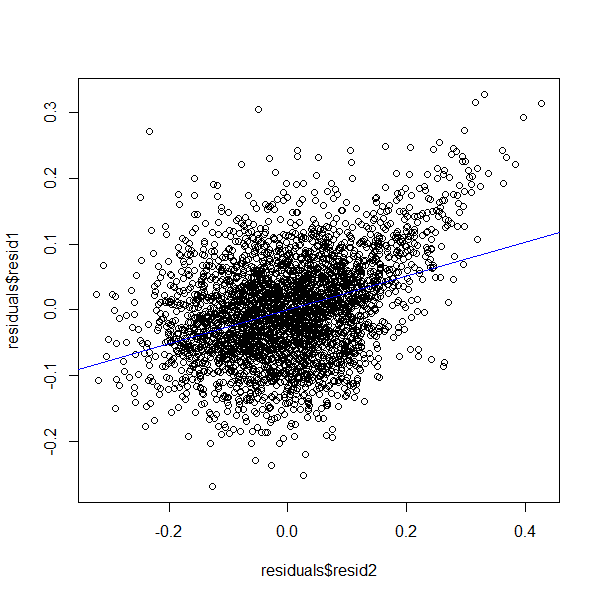
\includegraphics[width=.75\textwidth]{output/Reg4.png}
		\end{figure}
	\vspace{8cm} 
		\item Write the prediction equation. \\
			\noindent According to the output table, for every increase in one unit in the 'resid1' variable, there is a 0.257 unit increase in 'resid2'. This is shown via the equation: \\
		\noindent \textit{Y}$_{i}$ = 0.257\textit{X}$_{i}$
		
	\end{enumerate}
	
	\newpage	

\section*{Question 5}
\noindent What if the incumbent's vote share is affected by both the president's popularity and the difference in spending between incumbent and challenger? 
	\begin{enumerate}
		\item Run a regression where the outcome variable is the incumbent's \texttt{voteshare} and the explanatory variables are \texttt{difflog} and \texttt{presvote}.	\vspace{1cm} \\
			\noindent The following code was used to run the regression: \\
		\lstinputlisting[language=R, firstline=106, lastline=106]{code/PS3.R}
		\noindent From this, using Stargazer an output table was created (see Table 5)
		\begin{table}[!htbp] \centering 
			\caption{Voteshare and Difflog + Presvote} 
			\label{} 
			\begin{tabular}{@{\extracolsep{5pt}}lc} 
				\\[-1.8ex]\hline 
				\hline \\[-1.8ex] 
				& \multicolumn{1}{c}{\textit{Dependent variable:}} \\ 
				\cline{2-2} 
				\\[-1.8ex] & voteshare \\ 
				\hline \\[-1.8ex] 
				difflog & 0.036$^{***}$ \\ 
				& (0.001) \\ 
				& \\ 
				presvote & 0.257$^{***}$ \\ 
				& (0.012) \\ 
				& \\ 
				Constant & 0.449$^{***}$ \\ 
				& (0.006) \\ 
				& \\ 
				\hline \\[-1.8ex] 
				Observations & 3,193 \\ 
				R$^{2}$ & 0.450 \\ 
				Adjusted R$^{2}$ & 0.449 \\ 
				Residual Std. Error & 0.073 (df = 3190) \\ 
				F Statistic & 1,302.947$^{***}$ (df = 2; 3190) \\ 
				\hline 
				\hline \\[-1.8ex] 
				\textit{Note:}  & \multicolumn{1}{r}{$^{*}$p$<$0.1; $^{**}$p$<$0.05; $^{***}$p$<$0.01} \\ 
			\end{tabular} 
		\end{table}  
		\noindent From this regression, there was a significant result between the 'difflog' and 'presvote' variables, \textit{F}(1, 3190) = 1302.947, \textit{p} $<$ .01, with the adjusted R$^{2}$ = 0.449. This means that 44.9\% of the variance in the 'Voteshare' variable can be explained by the variance in the 'difflog' and 'Presvote' variables.
		\begin{figure}[h!]\centering
			\caption{\footnotesize Added-variable plots'}
			\label{fig:plots}
			\includegraphics[width=.75\textwidth]{output/Reg5.png}
		\end{figure}
		\vspace{12cm} 
		\item Write the prediction equation.	\vspace{1cm} \\
			\noindent According to the output table, for every increase in one unit in the 'voteshare' variable, there is a 0.036 unit increase in 'difflog', and a 0.257 unit increase in the 'presvote' variable. This is shown via the equation: \\
		\noindent \textit{Y}$_{i}$ = 0.449 + 0.036\textit{X}$_{i1}$ + 0.257\textit{X}$_{i2}$
		\item What is it in this output that is identical to the output in Question 4? Why do you think this is the case? \\
		\noindent The 'presvote' coefficient has an identical output to the 'resid2' coefficient in the regression carried out in question 4. This is because the presvote coefficient is derived from the variance in 'voteshare' that isn't explained by 'difflog'. Essentially, the coefficient is identical because it is controlling for the variance explained by the 'difflog' variable.
	\end{enumerate}




\end{document}
